%% ============================================================
%%  Presentación – Proyecto Grupo-2
%%  UK Road Safety: Traffic Accidents and Vehicles (2010–2017)
%%  Estilo: Geométrico / Editorial
%%  Compilar: pdflatex → biber → pdflatex × 2
%% ============================================================

\documentclass[aspectratio=169, 10pt]{beamer}

\usepackage[utf8]{inputenc}
\usepackage[T1]{fontenc}
\usepackage[spanish]{babel}
\usepackage{csquotes}
\usepackage{lmodern}
\usepackage{microtype}
\usepackage{graphicx}
\usepackage{tikz}
\usetikzlibrary{calc}
\usepackage{booktabs}
\usepackage{amsmath, amssymb}
\usepackage{xcolor}
\usepackage{tcolorbox}
\tcbuselibrary{skins, breakable}
\usepackage[backend=biber, style=apa, sorting=nyt]{biblatex}
\addbibresource{../referencias/referencias.bib}

%% ── Colores ─────────────────────────────────────────────────
\definecolor{Verde}{HTML}{1E222A}
\definecolor{VerdeM}{HTML}{252A34}
\definecolor{VerdeC}{HTML}{DED7D7}
\definecolor{Naranja}{HTML}{E69F00}
\definecolor{NaranjaC}{HTML}{E69F00}
\definecolor{Crema}{HTML}{FCFAF7}
\definecolor{GrisO}{HTML}{3A3A3A}
\definecolor{GrisC}{HTML}{888888}

%% ── Tema limpio ──────────────────────────────────────────────
\usetheme{default}
\usecolortheme{default}
\usefonttheme{professionalfonts}
\setbeamertemplate{navigation symbols}{}
\setbeamertemplate{frametitle}{}
\setbeamertemplate{footline}{}
\setbeamertemplate{headline}{}
\setbeamercolor{background canvas}{bg=Crema}
\setbeamercolor{normal text}{fg=GrisO}
\setbeamercolor{itemize item}{fg=Naranja}
\setbeamercolor{itemize subitem}{fg=VerdeC}
\setbeamertemplate{itemize item}{\small\raisebox{1pt}{$\blacktriangleright$}}
\setbeamertemplate{itemize subitem}{\small$\circ$}

%% ── Cabecera (sin texto con acentos dentro de TikZ) ─────────
\newcommand{\frameheader}[2]{%
  \begin{tikzpicture}[remember picture, overlay]
    \fill[Verde] (current page.north west)
      rectangle ([yshift=-1.15cm] current page.north east);
    \fill[Naranja] (current page.north west)
      rectangle ([xshift=0.45cm, yshift=-1.15cm] current page.north west);
    \fill[NaranjaC] ([xshift=-0.35cm] current page.north east)
      rectangle ([xshift=0cm, yshift=-1.15cm] current page.north east);
  \end{tikzpicture}%
  % Texto fuera de TikZ, posicionado con \makebox
  \begin{tikzpicture}[remember picture, overlay]
    \node[anchor=west, text=VerdeC, font=\tiny\bfseries]
      at ([xshift=0.65cm, yshift=-0.38cm] current page.north west)
      {\MakeUppercase{#1}};
    \node[anchor=west, text=white, font=\normalsize\bfseries]
      at ([xshift=0.65cm, yshift=-0.80cm] current page.north west)
      {#2};
  \end{tikzpicture}%
  \vspace{0.78cm}%
}

%% ── Pie de página ────────────────────────────────────────────
\newcommand{\myfooter}{%
  \begin{tikzpicture}[remember picture, overlay]
    \fill[Verde!90] (current page.south west)
      rectangle ([yshift=0.45cm] current page.south east);
    \fill[Naranja]
      ([xshift=-0.8cm] current page.south east)
      rectangle
      ([yshift=0.45cm] current page.south east);
  \end{tikzpicture}%
  \begin{tikzpicture}[remember picture, overlay]
    \node[anchor=west, text=VerdeC!70!white, font=\tiny]
      at ([xshift=0.3cm, yshift=0.22cm] current page.south west)
      {Grupo 2 \textperiodcentered{} CA0303 \textperiodcentered{} UCR};
    \node[anchor=east, text=white, font=\tiny\bfseries]
      at ([xshift=-1.0cm, yshift=0.22cm] current page.south east)
      {\insertframenumber/\inserttotalframenumber};
  \end{tikzpicture}%
}

%% ── Cajas tcolorbox ──────────────────────────────────────────
\tcbset{
  bloqueverde/.style={
    enhanced, boxrule=0pt, arc=3pt,
    colback=Verde!8, colframe=Verde, leftrule=4pt,
    top=8pt, bottom=6pt,
    fonttitle=\small\bfseries, coltitle=white,
    attach boxed title to top left={yshift=-2mm, xshift=4mm},
    boxed title style={colback=Verde, arc=2pt, boxrule=0pt}
  },
  bloquenaranja/.style={
    enhanced, boxrule=0pt, arc=3pt,
    colback=Naranja!8, colframe=Naranja, leftrule=4pt,
    top=8pt, bottom=6pt,
    fonttitle=\small\bfseries, coltitle=white,
    attach boxed title to top left={yshift=-2mm, xshift=4mm},
    boxed title style={colback=Naranja, arc=2pt, boxrule=0pt}
  },
  bloquementa/.style={
    enhanced, boxrule=0pt, arc=3pt,
    colback=VerdeC!15, colframe=VerdeC!60!Verde, leftrule=4pt,
    top=8pt, bottom=6pt,
    fonttitle=\small\bfseries, coltitle=white,
    attach boxed title to top left={yshift=-2mm, xshift=4mm},
    boxed title style={colback=VerdeC!60!Verde, arc=2pt, boxrule=0pt}
  }
}

%% ── Nodo de dato destacado ───────────────────────────────────
\newcommand{\datobig}[2]{%
  \begin{tikzpicture}
    \fill[Verde] (0,0) rectangle (2.8cm, 1.4cm);
    \fill[Naranja] (0,0) rectangle (0.15cm, 1.4cm);
  \end{tikzpicture}%
  % Superposición del texto con llapbox
  \llap{%
    \begin{minipage}[b][1.4cm][c]{2.8cm}
      \centering
      {\color{white}\large\bfseries #1}\\[-2pt]
      {\color{VerdeC}\tiny #2}
    \end{minipage}%
  }%
}

%% ── Bloque de color decorativo (sin texto) ───────────────────
\newcommand{\geoblocks}{%
  \begin{tikzpicture}
    \fill[Verde!15]   (0,0)    rectangle (3cm, 3.5cm);
    \fill[Naranja!25] (0.15cm,0.15cm) rectangle (1.2cm,1.2cm);
    \fill[VerdeC!35]  (1.4cm,2.1cm)   rectangle (2.9cm,3.3cm);
    \fill[Verde!40]   (0.15cm,1.4cm)  rectangle (0.9cm,2.0cm);
    \fill[NaranjaC!20](1.4cm,0.2cm)   rectangle (2.85cm,1.85cm);
  \end{tikzpicture}%
}

%% ============================================================
\begin{document}
%% ============================================================

%% ── PORTADA ──────────────────────────────────────────────────
\setbeamercolor{background canvas}{bg=Verde}
\begin{frame}[plain]
  \begin{tikzpicture}[remember picture, overlay]
    % Bloque naranja derecho
    \fill[Naranja]
      ([xshift=-4.2cm] current page.north east)
      rectangle (current page.south east);
    % Triángulo VerdeM
    \fill[VerdeM]
      ([xshift=-4.2cm] current page.north east) --
      ([xshift=-4.2cm, yshift=-3.5cm] current page.north east) --
      ([xshift=-7.5cm] current page.north east) -- cycle;
    % Rectángulo pequeño NaranjaC
    \fill[NaranjaC!60]
      ([xshift=-4.2cm, yshift=-3.5cm] current page.north east)
      rectangle ([xshift=-3.0cm, yshift=-4.1cm] current page.north east);
    % Línea VerdeC
    \draw[VerdeC, line width=1.2pt]
      ([xshift=1.2cm,  yshift=-4.8cm] current page.north west) --
      ([xshift=-4.5cm, yshift=-4.8cm] current page.north east);
  \end{tikzpicture}%
  % Texto de portada fuera de TikZ geométrico
  \begin{tikzpicture}[remember picture, overlay]
    \node[anchor=west, text=VerdeC, font=\tiny\bfseries, text width=9cm]
      at ([xshift=1.2cm, yshift=-2.0cm] current page.north west)
      {CA0303 \textperiodcentered{} ESTAD\'ISTICA ACTUARIAL I \textperiodcentered{} GRUPO 2};
    \node[anchor=west, text=white, font=\bfseries, text width=10cm]
      at ([xshift=1.2cm, yshift=-3.5cm] current page.north west)
      {Análisis de combinaciones de entorno en accidentes de tránsito del Reino Unido (2010-2017) mediante pruebas Chi-Cuadrado de independencia, V de Crámer y residuos estandarizados};
    
      \node[anchor=west, text=VerdeC, font=\small, text width=9cm]
      at ([xshift=1.2cm, yshift=-5.8cm] current page.north west)
      {Debbie Con Ortega     C32250 \\
       Ashly Garro Villanueva        C33198\\
       Emily Sanchéz Mancía  C27260\\
       Alessandro Umaña Vega C37963};
    \node[anchor=west, text=NaranjaC, font=\normalsize\bfseries]
      at ([xshift=1.2cm, yshift=-6.1cm] current page.north west)
      {};
    \node[anchor=center, text=white, font=\small\bfseries,
          text width=3.8cm, align=center]
      at ([xshift=-2.1cm, yshift=-5.5cm] current page.north east)
      {Universidad de Costa Rica };
  \end{tikzpicture}
\end{frame}
\setbeamercolor{background canvas}{bg=Crema}

%% ── CONTENIDO ────────────────────────────────────────────────
\begin{frame}[plain]
  \frameheader{}{Contenido}
  \myfooter
  \vspace{0.4cm}
  \begin{columns}[T]

    \begin{column}{0.50\textwidth}
      \renewcommand{\arraystretch}{1.6}
      \begin{tabular}{@{}c l l@{}}
        
        \textcolor{Verde}{\rule{7pt}{16pt}} &
        \textbf{1.} & \large Contexto y Pregunta de Investigaci\'on\\

        \textcolor{VerdeM}{\rule{7pt}{16pt}} &
        \textbf{2.} & \large Datos\\

        \textcolor{VerdeM}{\rule{7pt}{16pt}} &
        \textbf{3.} & \large Metodología y Resultados\\

        \textcolor{Naranja}{\rule{7pt}{16pt}} &
        \textbf{4.} & \large Conclusiones \\
      \end{tabular}

    \end{column}

    \begin{column}{0.42\textwidth}
      \centering
    \end{column}

  \end{columns}

\end{frame}

%% ============================================================
\section{Contexto y Pregunta de Investigaci\'on}
%% ============================================================

\begin{frame}[plain]
  \frameheader{01}{Contexto y Pregunta de Investigaci\'on}
  \myfooter
  \begin{columns}[T]
    \begin{column}{0.36\textwidth}
      \begin{tcolorbox}[bloqueverde, title=Contexto]
        \small
        \begin{itemize}
          \item jkdks
          \item kffjjdk
          \item kdkkd
        \end{itemize}
      \end{tcolorbox}
    \end{column}

    \begin{column}{0.6\textwidth}
      \begin{tcolorbox}[bloquenaranja, title=Pregunta de Investigación]
        \small 
        Qué patrones o combinaciones de patrones ocurren con mayor frecuencia 
        en los accidentes de tránsito del Reino Unido durante 2010-2017?
      \end{tcolorbox}
    \end{column}

  \end{columns}
\end{frame}

%% ============================================================
\section{Datos}
%% ============================================================

\begin{frame}[plain]
  \frameheader{02}{Datos -- Fuente y Variables}
  \myfooter
  \begin{columns}[T]
    \begin{column}{0.46\textwidth}
      \begin{tcolorbox}[bloqueverde, title=Fuente de datos]
        \small
        \text{UK Road Safety Accidents and Vehicles}\\[3pt]
        {\color{GrisC}\footnotesize Kaggle-Departamento de Transporte del Reino Unido}
      \end{tcolorbox}
      \vspace{8pt}
    \end{column}
    \begin{column}{0.50\textwidth}
      \begin{tcolorbox}[bloqueverde, title=Descripción de los datos]
        \begin{itemize}\small
          \item + 30  variables disponibles 
          \item 2,047,256 observaciones de accidentes 
          \item Período de observaciones: 2005-2017 
        \end{itemize}
      \end{tcolorbox}
    \end{column}
  \end{columns}

\end{frame}

%% ── Gráficos (2×2) ───────────────────────────────────────────

%% ============================================================
\section{Metodolog\'ia Propuesta}
%% ============================================================

\begin{frame}[plain]
  \frameheader{03}{Metodología propuesta}
  \myfooter
      \begin{tcolorbox}[bloqueverde, title=Pruebas de independencia $\chi^2$]
        \small
        \begin{itemize}
      \item \textbf{Chi-cuadrado:} evalúa la independencia entre variables.
        \[
        \chi^2=\sum_i\sum_j
        \frac{(n_{ij}-E_{ij})^2}{E_{ij}}
        \]
          $$ H_0: \text{Las variables son independientes vs } H_1: \text{ Las variables se relacionan}$$
        \item \textbf{V de Crámer:} mide la fuerza de la asociación.
        \[
        V=\sqrt{\frac{\chi^2}{N\min(I-1,J-1)}}
        \]

        \item \textbf{Residuos estandarizados:} identifican las combinaciones responsables de la asociación.
        \[
        r_{ij}=
        \frac{n_{ij}-E_{ij}}
        {\sqrt{E_{ij}(1-p_{i+})(1-p_{+j})}}
        \]
        \end{itemize}
      \end{tcolorbox}
\end{frame}

%% ============================================================
\section{Resultados}
%% ============================================================
\begin{frame}[plain]
  \frameheader{04}{Resultado}
  \myfooter
  \begin{center}
    \textbf{Superficie vial y límite de velocidad}
  \end{center}
  \begin{columns}[T]
    \begin{column}{0.5\textwidth}
      
\includegraphics[width=\textwidth]{Figuras/Residuos_superficie_lim.png}
    \end{column}

    \begin{column}{0.5\textwidth}
      \begin{itemize}
        \item Superficies húmedas, con hielo/escarcha, inundadas o con nieve → mucho más frecuentes de lo esperado en vías de alta velocidad.
        \item El clima no actúa solo, sino combinado con otras variables, confirma que la combinación (no cada factor por separado) 
        genera el exceso de riesgo \parencite{KARZAN2017}.
        \end{itemize}
    \end{column}
\end{columns}
\end{frame}

\begin{frame}[plain]
  \frameheader{04}{Resultados}
  \myfooter
  \begin{center}
    \textbf{Detalles de intersección y condiciones especiales}
  \end{center}
  \begin{columns}[T]
    \begin{column}{0.5\textwidth}
      
\includegraphics[width=\textwidth]{Figuras/Residuos_intresecc_obstaculos.png}
    \end{column}

    \begin{column}{0.5\textwidth}
      \begin{itemize}
        \item \textbf{Intersecciones reguladas:} fallas de semáforos/señalización.
        \item \textbf{Tramos rectos:} derrames accidentales, obras activas, asfalto defectuoso.
        \item Intersecciones concentran riesgo por convergencia de trayectorias, 
        en tramos rectos los conductores van más rápido \parencite{yannis_effectiveness_junctions}.
        \end{itemize}
    \end{column}
\end{columns}
\end{frame}
\begin{frame}[plain]
  \frameheader{04}{Resultados}
  \myfooter
  \begin{center}
    \textbf{Zona (urbana o rural) y momento del día}
  \end{center}
  \begin{columns}[T]
    \begin{column}{0.5\textwidth}
      
\includegraphics[width=\textwidth]{Figuras/Residuos_horaZona.png}
    \end{column}

    \begin{column}{0.5\textwidth}
      \begin{itemize}
\item Rural: pico en la mañana (rutina agrícola temprana).
\item Urbano: pico en la noche (ocio, salida laboral, poca visibilidad).
\item Los picos de siniestralidad se alinean con las rutinas sociales, no con el clima o infraestructura \parencite{HOSSEINIAN2012}.
        \end{itemize}
    \end{column}
\end{columns}
\end{frame}

\begin{frame}
  \myfooter
   \frameheader{02}{Datos -- Resultados Exploratorios}\\[1.8pt]
  \textbf{Condición de carretera}

  \centering
  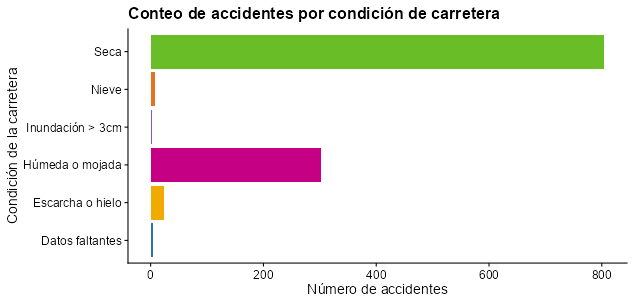
\includegraphics[width=0.65\textwidth]{../bitacoras/bitacora_2/figuras/frecuencia_condicion_calle.png}
\end{frame}


\begin{frame}[plain]
  \frameheader{04}{Resultados}
  \myfooter
  \begin{center}
    \textbf{Condición de la superficie de la vía y condición de luz}
  \end{center}
  \begin{columns}[T]
    \begin{column}{0.5\textwidth}
      
\includegraphics[width=\textwidth]{Figuras/Residuos_superficie_luz.png}
    \end{column}

    \begin{column}{0.5\textwidth}
      \begin{itemize}
\item \textbf{Mayor frecuencia:} día + superficie seca (mayor flujo vehicular).
\item \textbf{Patrones:} mojado/inundado → oscuridad con o sin luz artificial y hielo/escarcha → oscuridad sin alumbrado.
\item  Pérdida de fricción + menor agudeza visual del conductor = mayor riesgo \parencite{KARZAN2017}.
        \end{itemize}
    \end{column}
\end{columns}
\end{frame}

\begin{frame}[plain]
  \frameheader{04}{Resultados}
  \myfooter
  \begin{center}
    \textbf{Superficie y tipo de carretera}
  \end{center}
  \begin{columns}[T]
    \begin{column}{0.5\textwidth}
      
\includegraphics[width=\textwidth]{Figuras/Residuos_superficie_tipodevia.png}
    \end{column}

    \begin{column}{0.5\textwidth}
      \begin{itemize}
\item \textbf{Mayor riesgo:} hielo, nieve o inundaciones localizadas.
\item El problema no es solo la superficie, sino la falta de ajuste por parte 
del conductor (velocidad sostenida sin anticipar el cambio de fricción) \parencite{KARZAN2017}.
      \end{itemize}
    \end{column}
\end{columns}
\end{frame}


\begin{frame}[plain]
  \frameheader{04}{Resultados}
  \myfooter
  \begin{center}
    \textbf{Condición de luz y tipo de carretera}
  \end{center}
  \begin{columns}[T]
    \begin{column}{0.5\textwidth}
      
\includegraphics[width=\textwidth]{Figuras/Residuos_ilum_via.png}
    \end{column}

    \begin{column}{0.5\textwidth}
      \begin{itemize}
\item Vías dobles en oscuridad total → accidentes muy superiores a lo esperado.
\item A alta velocidad sin alumbrado, la distancia de frenado excede el alcance 
visible de los faros, reduciendo el tiempo de reacción \parencite{TAYLOR2000}.
      \end{itemize}
    \end{column}
\end{columns}
\end{frame}


\begin{frame}
  \myfooter
   \frameheader{02}{Datos -- Resultados Exploratorios}\\[1.8pt]
  \textbf{Condición de carretera}

  \centering
  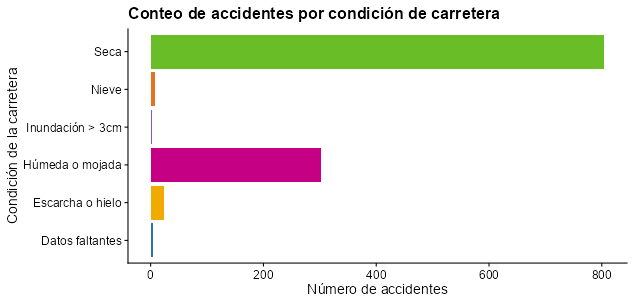
\includegraphics[width=0.65\textwidth]{../bitacoras/bitacora_2/figuras/frecuencia_condicion_calle.png}
\end{frame}




%% ── REFERENCIAS ──────────────────────────────────────────────
\begin{frame}[plain, allowframebreaks]
  \frameheader{}{Referencias}
  \myfooter
  \printbibliography[heading=none]
\end{frame}

%% ── CIERRE ───────────────────────────────────────────────────
\setbeamercolor{background canvas}{bg=Verde}
\begin{frame}[plain]
  \begin{tikzpicture}[remember picture, overlay]
    \fill[Naranja]
      ([xshift=-3.5cm] current page.north east)
      rectangle (current page.south east);
    
    \draw[VerdeC, line width=1pt]
      ([xshift=-6.5cm, yshift=-0.3cm] current page.center) --
      ([xshift=0.4cm,  yshift=-0.3cm] current page.center);
  \end{tikzpicture}
  \begin{tikzpicture}[remember picture, overlay]
    \node[text=white, font=\Huge\bfseries, anchor=center]
      at ([xshift=-3cm, yshift=1.0cm] current page.center)
      {¡Gracias!};
    \node[text=VerdeC, font=\small, anchor=center]
      at ([xshift=-3cm, yshift=0.1cm] current page.center)
      {Grupo 2 \textperiodcentered{} CA0303 \textperiodcentered{} UCR};
    \node[text=white, font=\small\bfseries, align=center, anchor=center]
      at ([xshift=-1.75cm] current page.east |- current page.center)
      {Escuela de\\Matem\'atica\\UCR};
  \end{tikzpicture}
\end{frame}

\end{document}